\documentclass[a4paper,14pt]{extarticle}

\usepackage[top=2.5cm, bottom=2.5cm, left=2.5cm, right=2.5cm]{geometry}
\usepackage[utf8]{inputenc}
\usepackage[russian]{babel}
\usepackage[final]{graphicx}
\usepackage{caption}
\usepackage{subcaption}
\usepackage{chngcntr}
\usepackage{amsmath}
\usepackage{amsfonts}
\usepackage{pgfplots}
\usepackage{pgfplotstable}
\usepgfplotslibrary{fillbetween}
\usepackage{float}
\usepackage{lipsum}% http://ctan.org/pkg/lipsum
\usepackage{multicol}% http://ctan.org/pkg/multicol
\usepackage{hhline}
\usepackage{tabularx}
\usepackage{tikz,xcolor}
\usepackage{tkz-graph}
\usepackage{float}
\usepackage{mathtools}
\usepackage{todonotes}
\usepackage{listings}
\usepackage{epstopdf}
\usepackage{epsfig}
\usepackage[makeroom]{cancel}
\usepackage{subcaption}

\usetikzlibrary{arrows, petri, topaths}

\counterwithin{figure}{section}
\counterwithin{equation}{section}
\counterwithin{table}{section}

\DeclareMathOperator*{\argmin}{arg\,min}
\DeclareMathOperator*{\argmax}{arg\,max}
\DeclareMathOperator{\sinc}{sinc}

\definecolor{mygreen}{RGB}{28,172,0} % color values Red, Green, Blue
\definecolor{mylilas}{RGB}{170,55,241}

\lstset{language=Matlab,%
  %  basicstyle=\color{red},
    breaklines=true,%
    morekeywords={matlab2tikz,ylim,xlim,square,ones,double},
    keywordstyle=\color{blue},%
    morekeywords=[2]{1}, keywordstyle=[2]{\color{black}},
    identifierstyle=\color{black},%
    stringstyle=\color{mylilas},
    commentstyle=\color{mygreen},%
    showstringspaces=false,%without this there will be a symbol in the places where there is a space
    numbers=left,%
    numberstyle={ \color{black}},% size of the numbers
    numbersep=15pt, % this defines how far the numbers are from the text
    emph=[1]{for,end,break,switch,case,otherwise},emphstyle=[1]\color{red}, %some words to emphasise
    %emph=[2]{word1,word2}, emphstyle=[2]{style},    
}


\begin{document}
\begin{titlepage}
\centering 
{\bfseries Санкт-Петербургский Политехнический Университет} \\
Институт компьютерных наук и технологий \\
Кафедра компьютерных систем и программных технологий \\
\vspace{5cm}
{\centering \textbf{Отчёт по лабораторной работе №3} \\ 
\vspace{0.15cm}
\textbf{Дисциплина}: Телекоммуникационные технологии \\
\vspace{0.15cm}
\textbf{Тема}: Линейная фильтрация.} \\
\vspace{4cm}
\hfill {\bfseries Работу выполнил студент}  \\
\hfill гр. 33501/4 Леженин Ю.И. \\
\hfill {\bfseries Преподаватель}  \\
\hfill Богач Н.В.
\vfill
Санкт-Петербург \\
{\large \today\par}
\end{titlepage}

\section{Цель работы.}

Изучить воздействие ФНЧ на тестовый сигнал с шумом.

\section{Постановка задачи.} 

Cгенерировать гармонический сигнал с шумом
и синтезировать ФНЧ. Получить сигнал во временной и частотной
областях до и после фильтрации. Сделать выводы о воздействии
ФНЧ на спектр сигнала.

\section{Ход работы.}

\subsection{Линейные цепи.}
Преобразование непрерывных сигналов в линейных цепях с постоянными параметрами может быть описано с помощью линейных дифференциальных уравнений с постоянными коэффициентами.

При прохождении гармонического сигнала через такую цепь меняется его амплитуда и фаза: 
\begin{equation*}
x(t) = A_x e^{j (2 \pi f t + \phi_x)} \rightarrow y(t) = A_y e^{j (2 \pi f t + \phi_y)}.
\end{equation*} 
Отношение выходного сигнала ко входному произвольной частоты называется частотной характеристикой (ЧХ):
\begin{equation*}
G(f) = \frac{A_y}{A_x} e^{j (\phi_y - \phi_x)} = |G(f)|e^{j \phi(f)}.
\end{equation*}
Модуль $|G(f)|$ называется амплитудно-частотная характеристика, $\phi(f)$ -- фазо-частотная характеристика.
Реакция цепи $g(t)$ на единичный $\delta$-импульс называется импульсная характеристика (ИХ).

При прохождении через цепь произвольного сигнала $x(t)$, спектр выходного сигнала $y(t)$ имеет вид
\begin{equation*}
Y(f) = X(f) G(f).
\end{equation*}
Согласно теореме о свертки выходной сигнал может быть найден как 
\begin{equation*}
y(t) = x(t) * g(t) = \int_{-\infty}^{t} x(t')g(t - t') dt'.
\end{equation*}   


\subsection{Фильтры.}
Линейные цепи широко используются в качестве фильтров. Фильтры -- это устройства, целенаправленным образом изменяющие спектры сигналов. Фильтрация позволяет повысить отношение полезного сигнала к шумам и помехам.

Фильтры часто классифицируют по виду частотной характеристики, выделяют четыре основных типа:
\begin{itemize}
\setlength\itemsep{-0.4em}
\item фильтр нижних частот (ФНЧ),
\item фильтр верхних частот (ФВЧ),
\item фильтр полосно-пропускающий (ФПП),
\item фильтр полосно-заграждающий (ФПЗ).
\end{itemize}
Частотные характеристики для идеальных фильтров, относящихся к перечисленным типам, приведены на рисунке \ref{fs}.


\begin{figure}[H]
\centering
\begin{subfigure}[b]{0.49\textwidth}
\includegraphics[width=1\textwidth]{lpf.eps}
\captionsetup{justification=centering,margin=1cm}
\caption{ФНЧ}
\end{subfigure}
\begin{subfigure}[b]{0.49\textwidth}
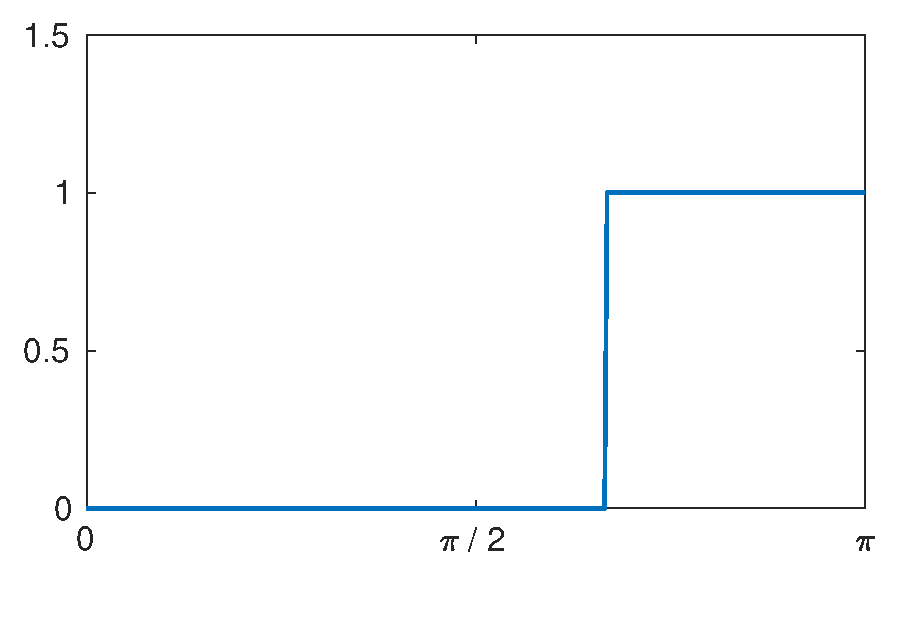
\includegraphics[width=1\textwidth]{hpf.eps}
\captionsetup{justification=centering,margin=1cm}
\caption{ФВЧ}
\end{subfigure}
\begin{subfigure}[b]{0.49\textwidth}
\includegraphics[width=1\textwidth]{bpf.eps}
\captionsetup{justification=centering,margin=1cm}
\caption{ФПП}
\end{subfigure}
\begin{subfigure}[b]{0.49\textwidth}
\includegraphics[width=1\textwidth]{bsf.eps}
\captionsetup{justification=centering,margin=1cm}
\caption{ФПЗ}
\end{subfigure}
\caption{Частотные характеристики идеальных фильтров.}
\label{fs}
\end{figure}

Идеальная характеристика представляет собой прямоугольную функцию, соответствующая импульсная характеристика представляет собой функцию $\sinc(t)$. Данная функция определена на интервале $[-\infty, \infty]$, что делает физическую реализацию невозможной. Для получения фильтра с частотной характеристикой приближенной к идеальной существует множество различных техник синтеза. 

Существует два типа архитектуры цифровых фильтров. Фильтры с конечной импульсной характеристикой (КИХ) порядка $l$ строятся по принципу 
\begin{equation*}
y[n] = a_0\,x[n] + a_1\,x[n-1] + \dots + a_l\,x[n-l].
\end{equation*} 
Фильтры с бесконечной импульсной характеристикой (БИХ) включают рекурсивные зависимости:
\begin{equation*}
\begin{split}
y[n] = a_0\,x[n] + a_1\,x[n-1] + \dots + a_l\,x[n-l] + \\ + b_1\,y[n-1] + \dots + b_m\,y[n-m].
\end{split}
\end{equation*} 
КИХ-фильтры наиболее просты для синтеза и применения, они всегда имеют линейную ФЧХ. БИХ-фильтры требуют соблюдение условий устойчивости, а задержка ФЧХ, как правило, нелинейна.


\subsection{Фильтрация сигнала.}

Для демонстрации работы фильтров был смоделирован гармонический  сигнал $x(t) = sin(2\pi \, 5 t) - 0.5 cos(2\pi \, 2.5 t)$. К исходному сигналу был добавлен белый шум распределенный по закону Гаусса. Исходный и зашумленные сигналы приведены на рисунке \ref{sig}.
 
\begin{figure}[H]
\centering
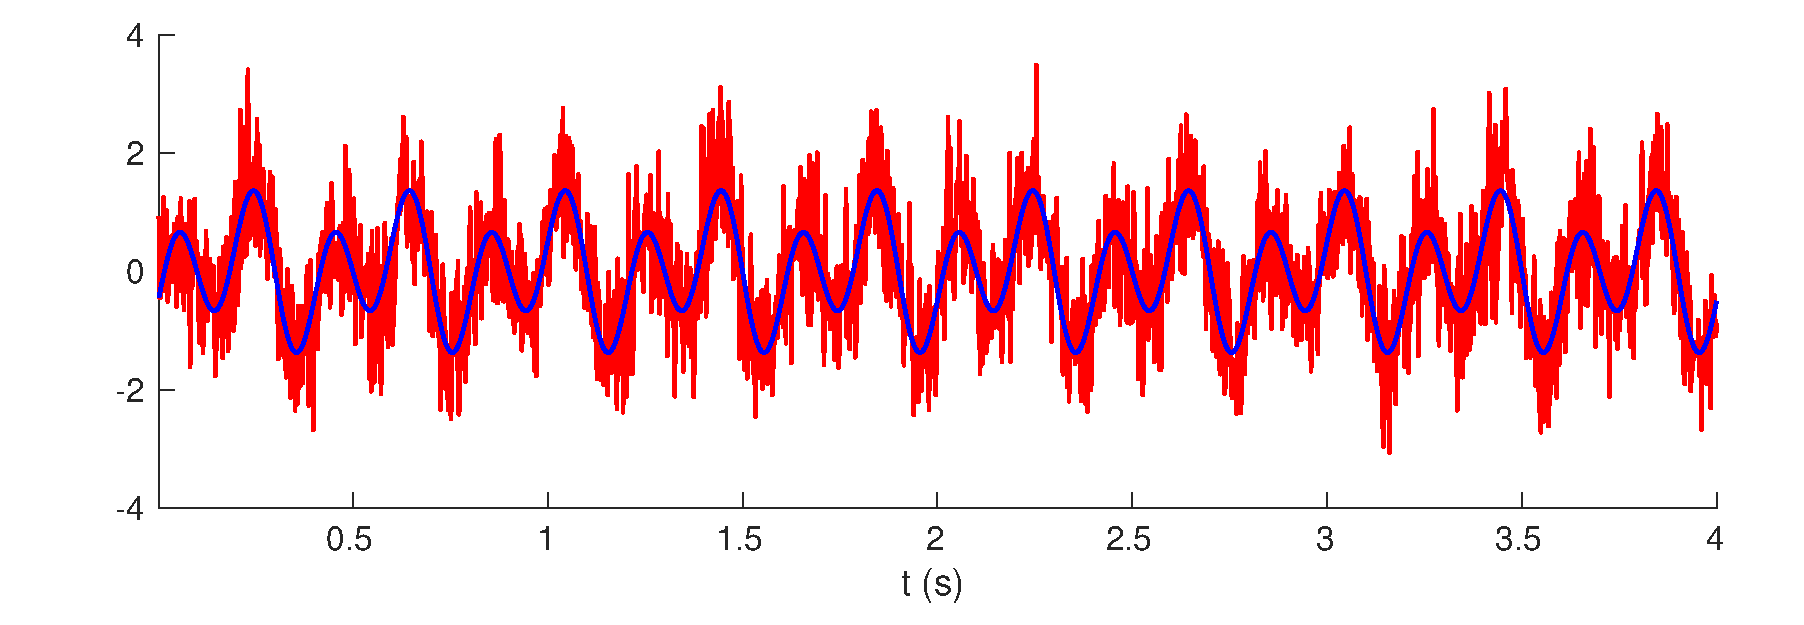
\includegraphics[width=\textwidth]{signal.eps}
\captionsetup{justification=centering,margin=0.5cm}
\caption{Сигнал вида $x(t) = sin(2\pi \, 5 t) - 0.5 cos(2\pi \, 2.5 t)$ и тот же сигнал с наложенным белым шумом. Отношение сигнал/шум 3 Дб.}
\label{sig}
\end{figure}

В частотном представлении сигналу соответствует 4 импульса на частотах -5 Гц и 5 Гц, -2.5 Гц и 2.5 Гц. Для зашумленного сигнала спектр содержит шум распределенный равномерно по частотам. Спектр 
исходного и зашумленного сигнала приведены на рисунке \ref{spec}.

\begin{figure}[H]
\centering
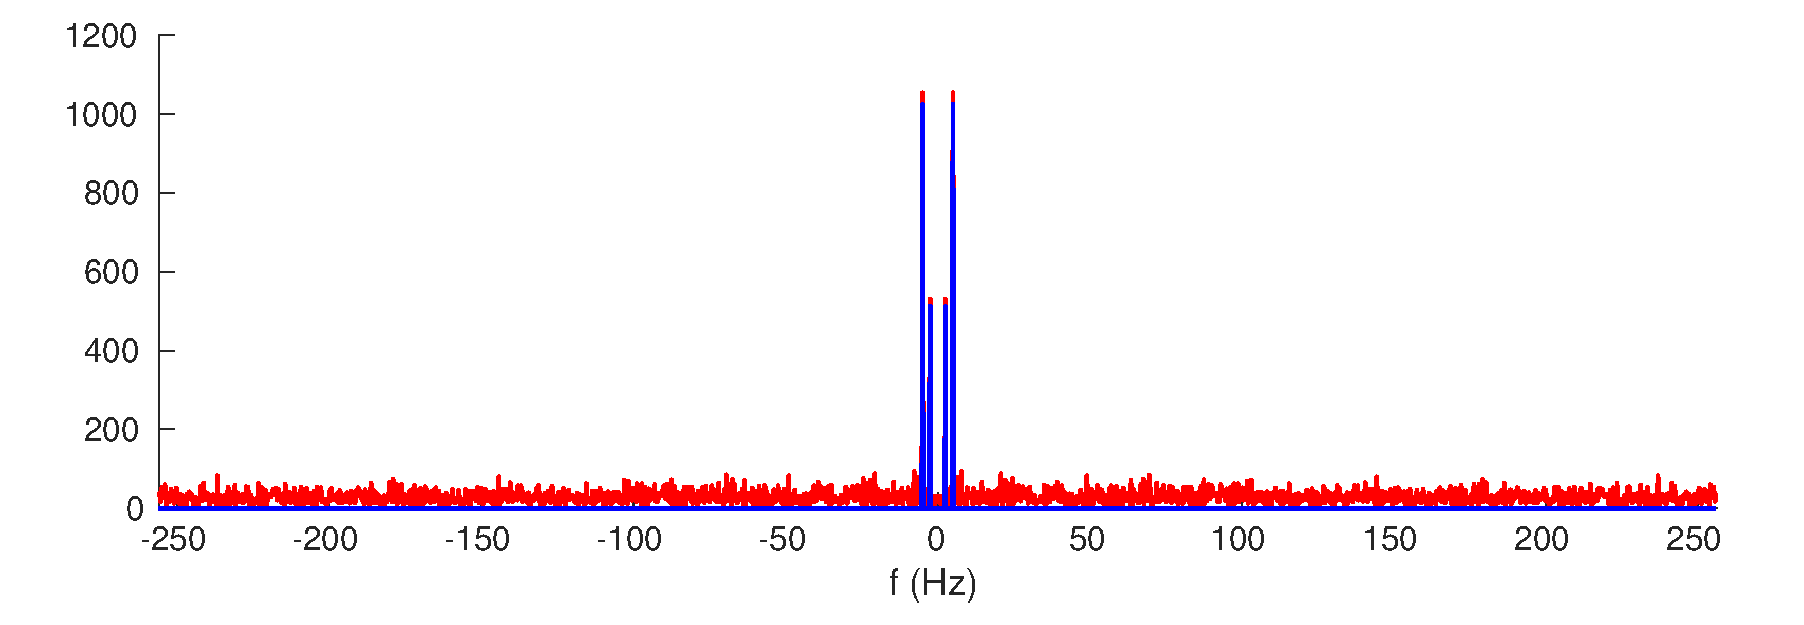
\includegraphics[width=1\textwidth]{spectrum.eps}
%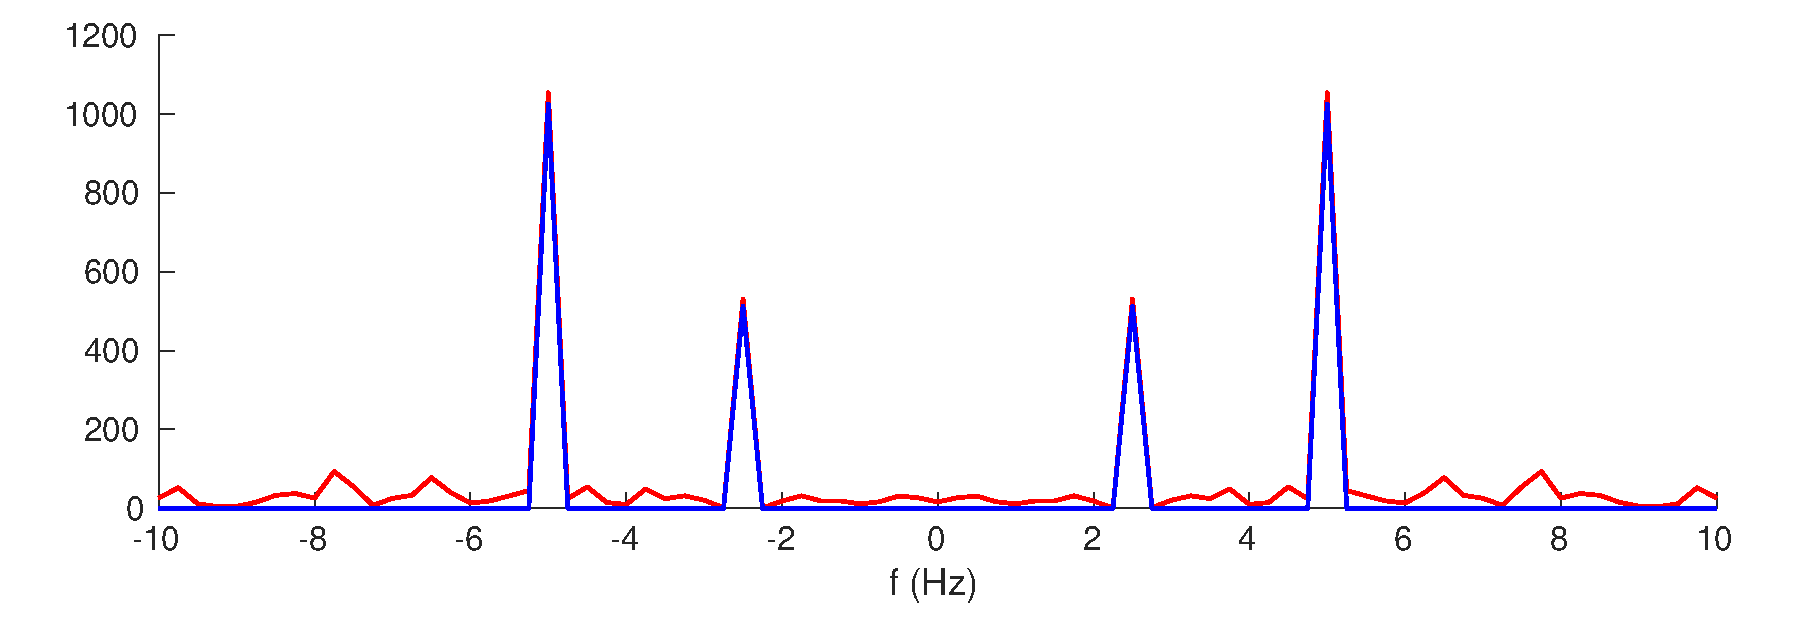
\includegraphics[width=1\textwidth]{spectrum_zoomed.eps}
\captionsetup{justification=centering,margin=0.5cm}
\caption{Cпектр сигнала вида $x(t) = sin(2\pi \, 5 t) - 0.5 cos(2\pi \, 2.5 t)$ и спектр того же сигнала с наложенным белым шумом. \\Отношение сигнал/шум 3 Дб.}
\label{spec}
\end{figure}

Для удаления шума был синтезирован фильтр с использованием окна Каизера. Граница полосы пропускания находится на частоте $F_{pass}$ = 6 Гц, а полосы заграждения -- частоте $F_{stop}$ = 12 Гц, допустимая амплитуда отклонений в полосе пропускания $A_{pass}$ = 1 Дб, уменьшение амплитуды в полосе заграждения $A_{stop}$ = -40 Дб. Полученный в результате синтеза фильтр 191 порядок. Частотная и импульсная характеристики фильтра приведены на рисунке \ref{mag_res}.

\begin{figure}[H]
\centering
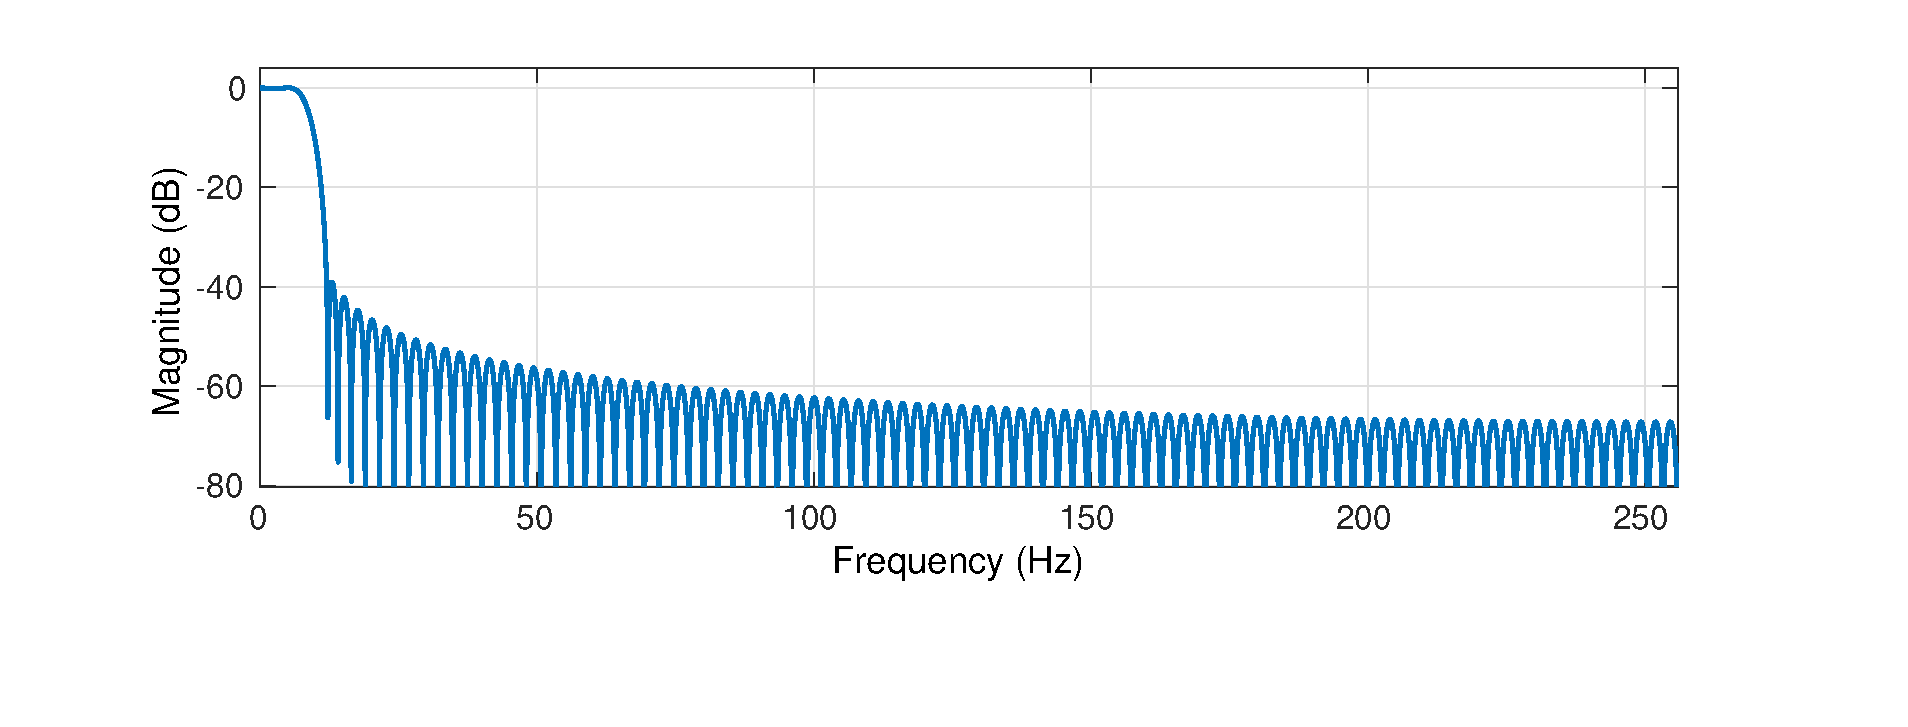
\includegraphics[width=0.9\textwidth]{mag_resp.eps}
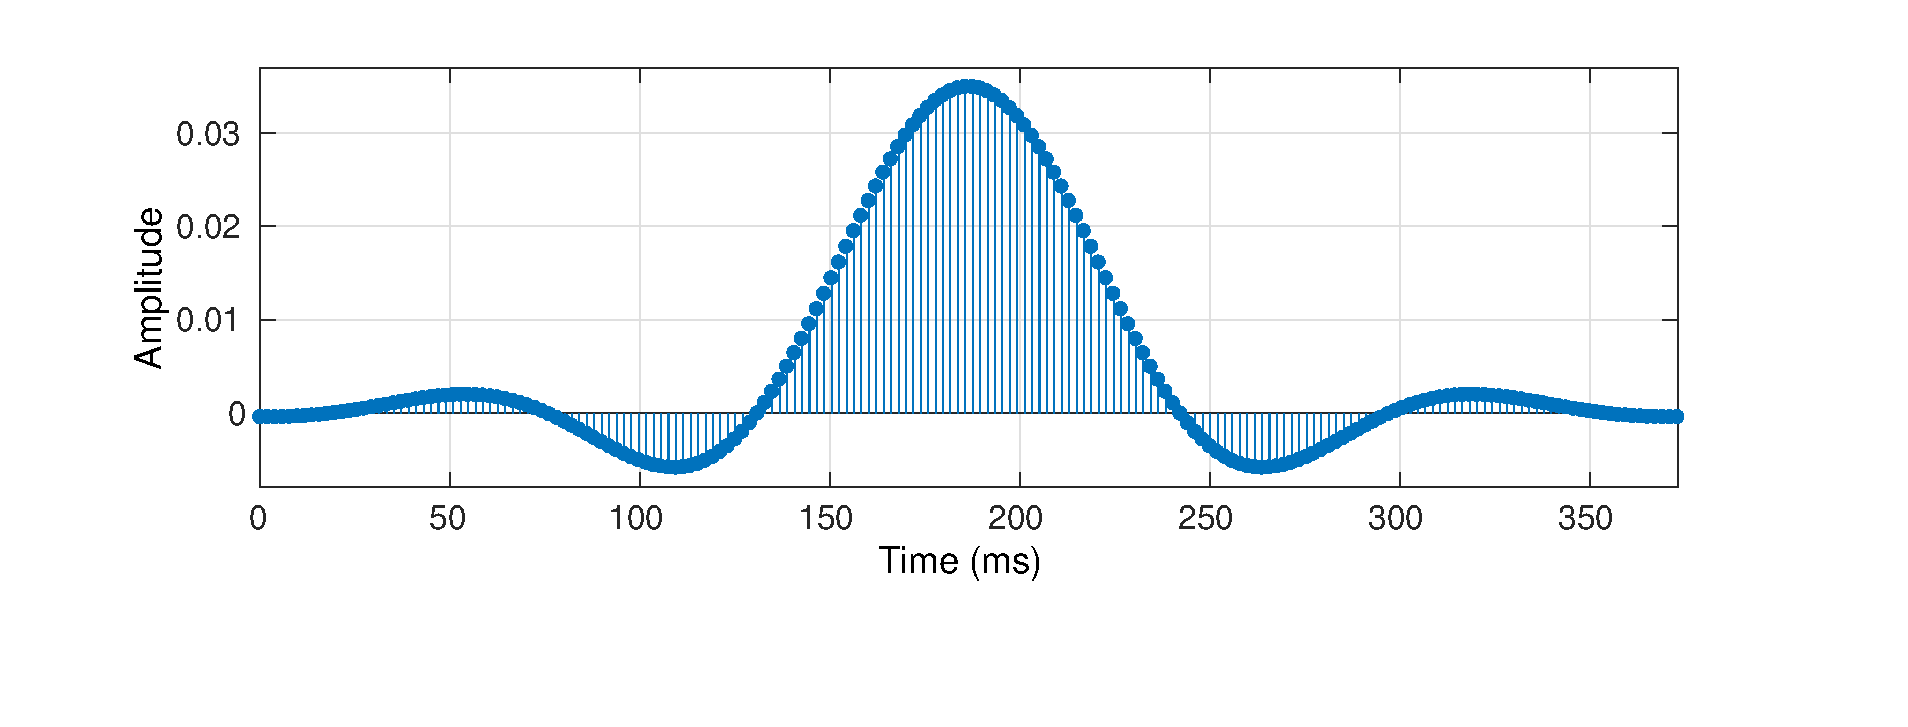
\includegraphics[width=0.9\textwidth]{imp_resp.eps}
\captionsetup{justification=centering,margin=0.5cm}
\caption{Амплитудно-частотная и импульсная характеристики синтезированного фильтра с окном Кайзера 191 порядка. }
\label{mag_res}
\end{figure}
%
%\begin{figure}[H]
%\centering
%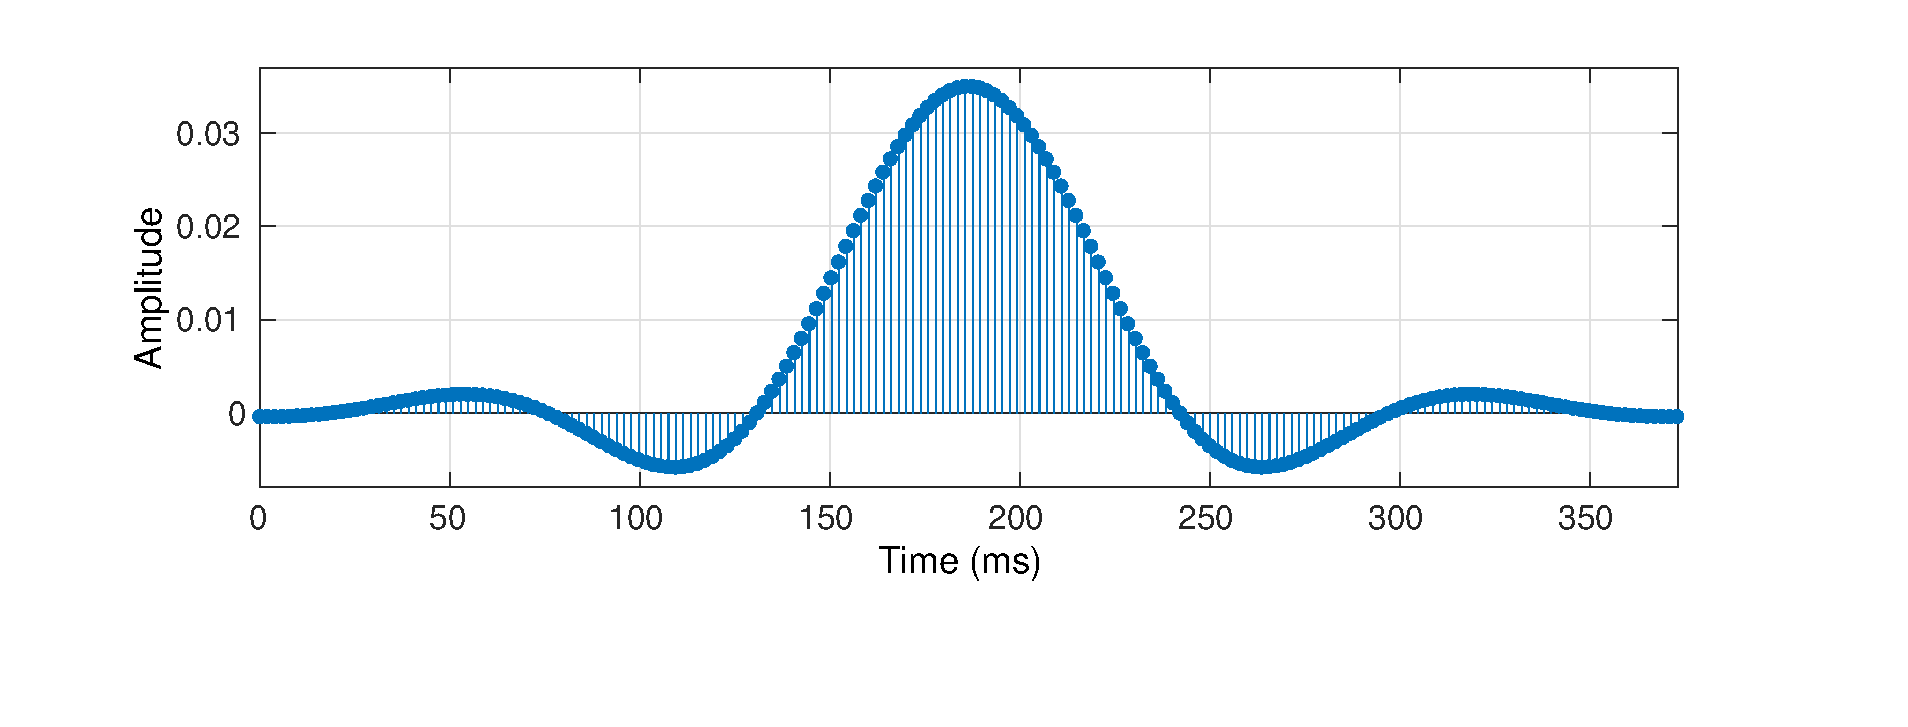
\includegraphics[width=1\textwidth]{imp_resp.eps}
%\captionsetup{justification=centering,margin=0.5cm}
%\caption{Импульсная характеристика синтезированного фильтра с окном Кайзера 191 порядка.}
%\label{imp_res}
%\end{figure}

После прохождения через фильтр сигнал имеет задержку, длительность которой зависит от порядка фильтра. Шум на высоких частотах отсутствует, однако в полосе пропускания фильтра шум сохраняется, выходной сигнал имеет искажения. Исходный сигнал и выход фильтра приведены на рисунке \ref{sig_filt}. Спектр исходного сигнала и спектр сигнала с выхода фильтра приведены на рисунке \ref{spec_filt}. 

\begin{figure}[H]
\centering
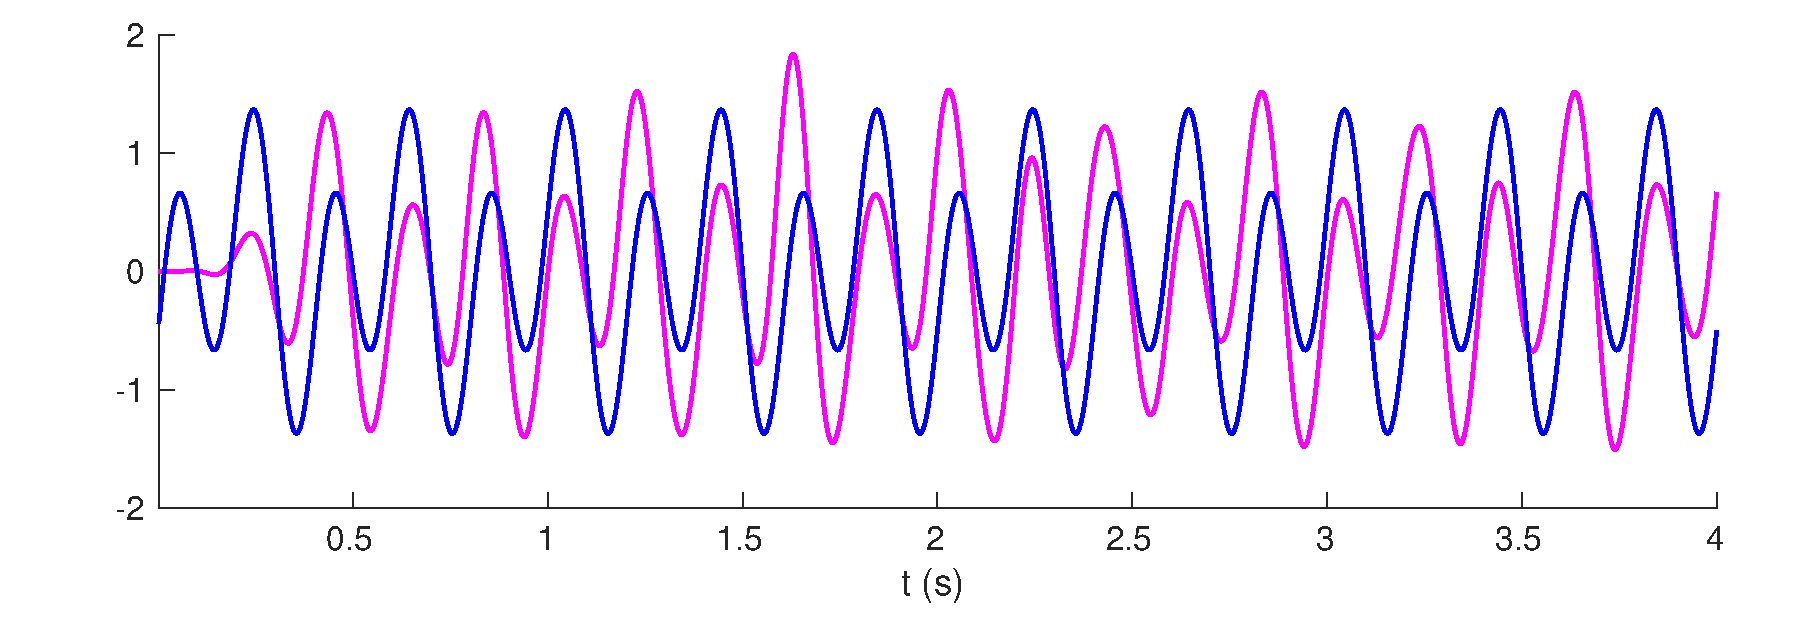
\includegraphics[width=1\textwidth]{signal_filtered.eps}
\captionsetup{justification=centering,margin=0.5cm}
\caption{Сигнал вида $x(t) = sin(2\pi \, 5 t) - 0.5 cos(2\pi \, 2.5 t)$ и сигнал с выхода фильтра с окном Кайзера 191 порядка.}
\label{sig_filt}
\end{figure}

\begin{figure}[H]
\centering
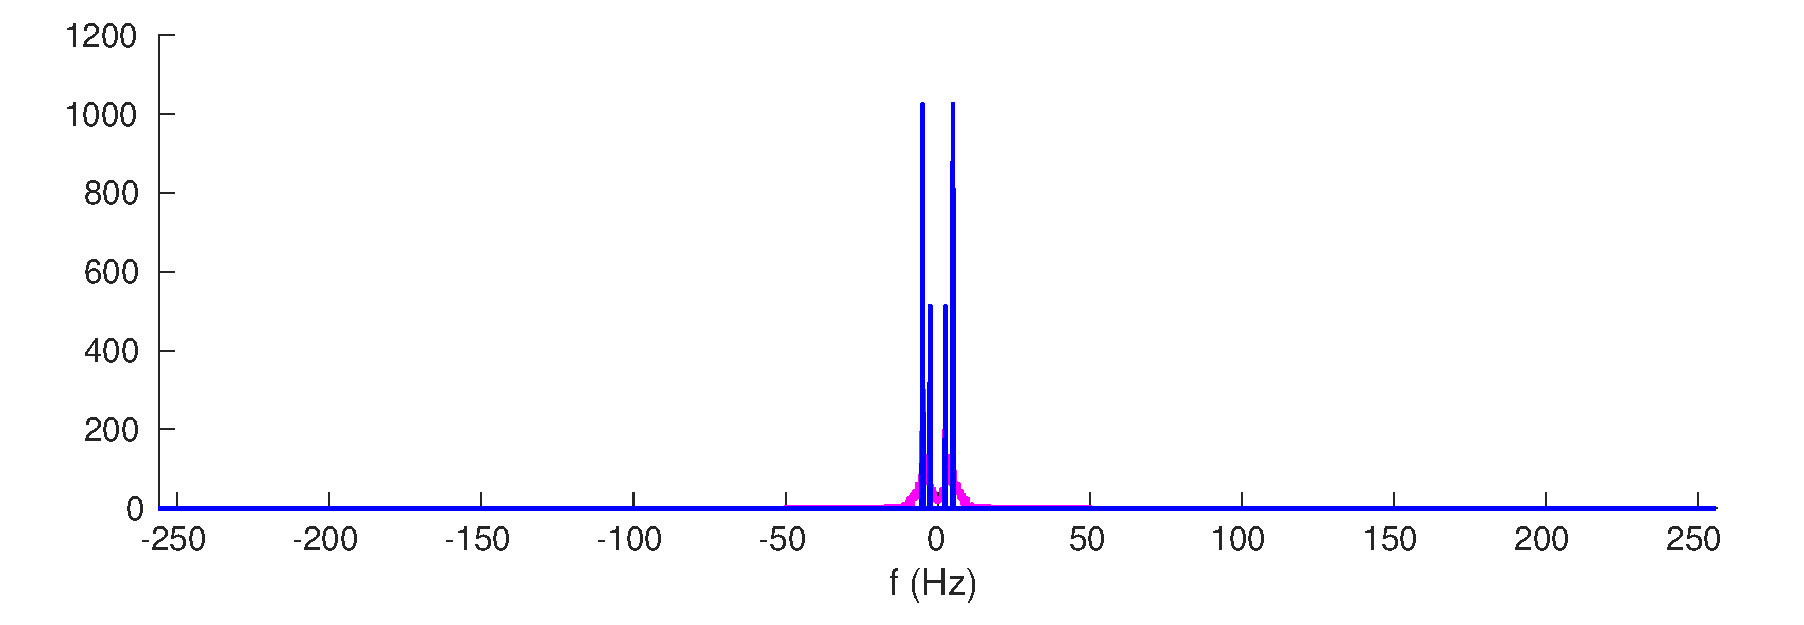
\includegraphics[width=1\textwidth]{spectrum_filtered.eps}
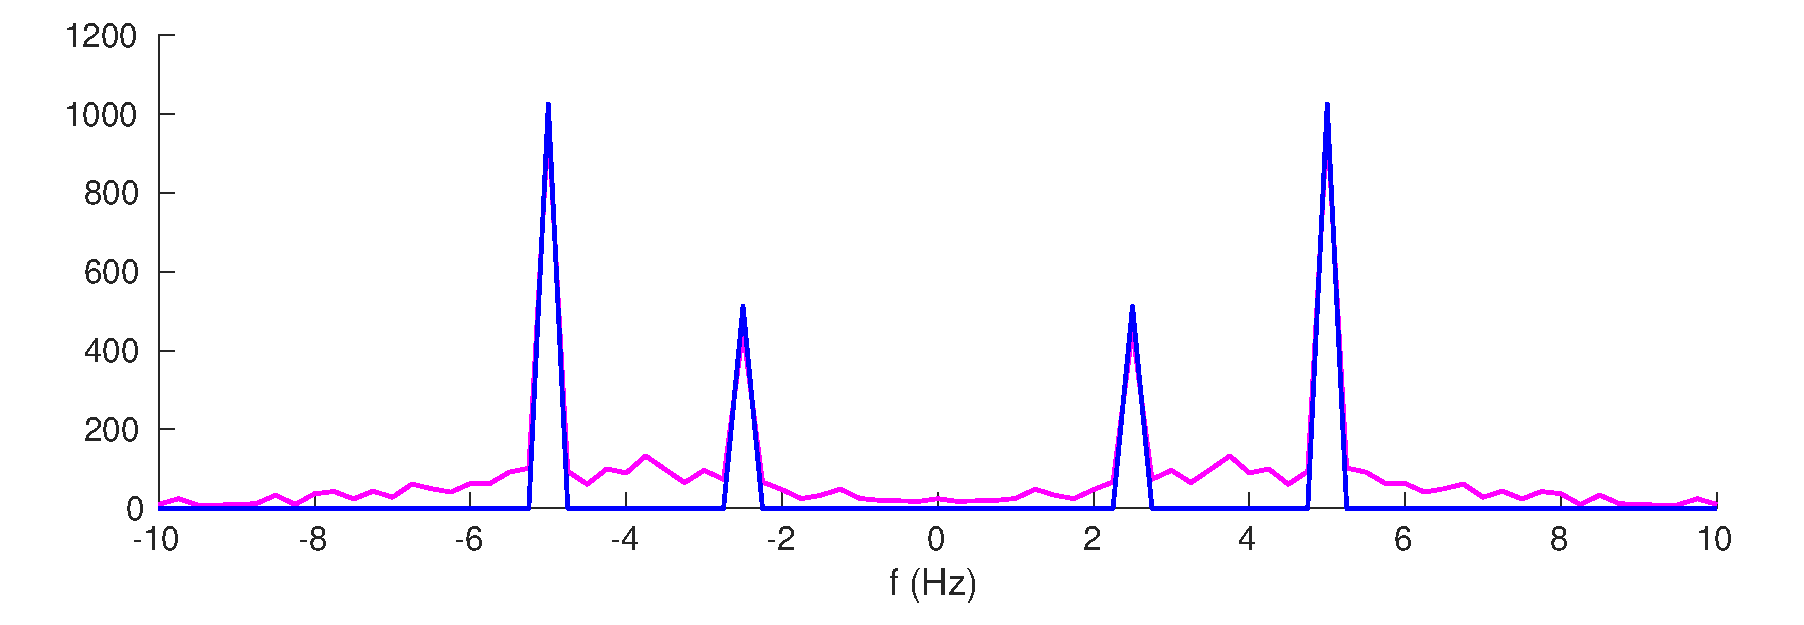
\includegraphics[width=1\textwidth]{spectrum_filtered_zoomed.eps}
\captionsetup{justification=centering,margin=0.5cm}
\caption{Cпектр сигнала вида $x(t) = sin(2\pi \, 5 t) - 0.5 cos(2\pi \, 2.5 t)$ и спектр сигнала с выхода фильтра с окном Кайзера 191 порядка.}
\label{spec_filt}
\end{figure}

\section{Выводы.}

Линейный цепи позволяют осуществлять фильтрацию сигнала, т.е. целенаправленным образом менять спектр сигнала. Это позволяет повысить отношение полезного сигнала к шумам и помехам.

По виду амплитудно-частотной характеристики фильтры делятся на 4 типа: ФНЧ, ФВЧ, ФПП, ФПЗ.
По виду импульсной характеристики выделяют КИХ-фильтры и БИХ-фильтры.



\section{Приложение.}

\lstinputlisting[frame=single, caption=Программа для генерации и фильтрации сигналов.]{lab3_script.m}


\end{document}